% Chapter Template

\chapter{Solution Design} % Main chapter title

\label{Chapter4} % Change X to a consecutive number; for referencing this chapter elsewhere, use \ref{ChapterX}

\section{General Approach} \label{sec:generalApproach}

With the aim of complete the specific objectives and thus the main one, all of them mentioned in Sec.\ref{sec:thesisGoals}, a workflow was designed. This work flow contains five stages.

\begin{enumerate}
	\item The applications were instrumented using \textbf{InstruAPK.}
	\item The exploration was made using Droidbot, Monkey, RIP and Firebase Testlab
	\item The coverage measurement was made using \textbf{CoverageAnalyzer (CA).}
	\item Summarize data. Total number of unique methods called during all ten executions, reporting only the first time they were called.
	\item Understanding data, computing statistics, creating graphs, extract insights and concluding.
\end{enumerate}

Stages 2. and 3. were repeated 10 times for every application that was selected, that leaded to the stage iv. The multiple executions are intending to get average values as well as better comparable results along the different exploration tools.

\begin{figure}[h]
\centering
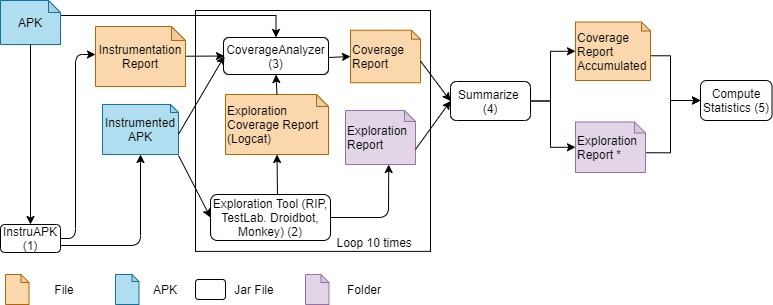
\includegraphics[width=0.8\textwidth]{../Figures/workflow.jpg}
\label{fig:workflow}
\caption{Main Workflow}
\end{figure}


explicar el workflow de cómo se obtuvieron los resultados.

\textbf{APK processing.} 

In order to measure the method coverage reached by an exploration tool in one application, there is the need to know how many methods there are in the application and how many methods were called during the exploration. To achieve that, \textbf{InstruAPK.} and \textbf{CoverageAnalyzer (CA).} were developed.
%TODO citate InstruAPK repository
%TODO citate CA repository

\section{InstruAPK}

Instrumentation tool developed mainly for this study. This tool uses APKTool, a known Java application that allows inverse engineering in Android apps, allowing applications' instrumentation without the need of recompiling their source code. APKTool decodes the apk and the result is the smali representation of the app source code, These smali files are analysed in order to find all the methods to be instrumented and then, the log code is injected at the very beginning of each method. Its important to notice that no external libraries methods are instrumented. InstruAPK only search for methods following the android project structure that uses the application package name to store the application source code.

\begin{figure}[h]
\centering
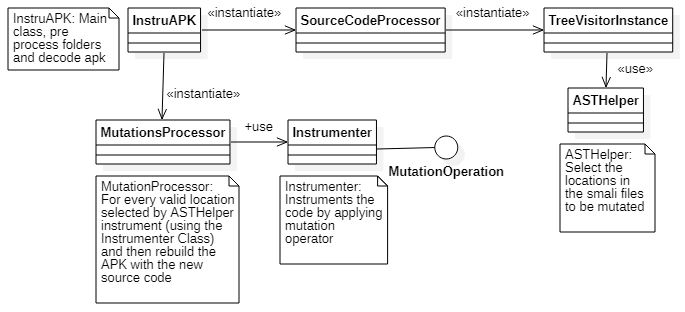
\includegraphics[width=0.8\textwidth]{../Figures/ClassDiagramInstruAPK.jpg}
\label{fig:instruAPK}
\caption{Class Diagram InstruAPK}
\end{figure}

%TODO explain the architecture and the tool in more detail, do not throw the image and just that.
\section{Coverage Analyser (CA)}

Java Application created mainly for this study. This tool extracts all data from the log lines injected by InstruAPK. When an instrumented application is ran, the logcat will contain the log lines with all the data. The logcat is stored in a txt file and that is what CA uses as its input. As CA depends totally on the information provided by InstruAPK, CA can be seen as a complement of it, rather than an separate application.

\begin{figure}[h]
\centering
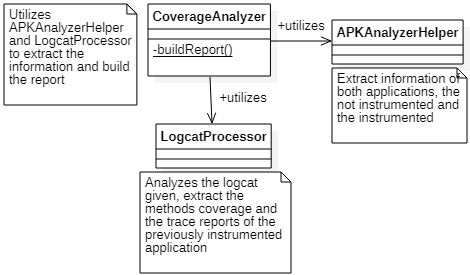
\includegraphics[width=0.8\textwidth]{../Figures/ClassDiagramCA.jpg}
\label{fig:ca}
\caption{Class Diagram Coverage Analyser}
\end{figure}
%TODO explain the architecture and the tool in more detail, do not throw the image and just that.